%\documentclass[notes,11pt,aspectratio=169]{beamer}
\documentclass[11pt,aspectratio=169]{beamer}
\usetheme{auriga} %Themes http://www.hartwork.org/beamer-theme-matrix/
\usecolortheme{auriga}


\definecolor{red}{RGB}{255, 0, 0}
\definecolor{blue}{RGB}{0, 118, 186}
\definecolor{green}{RGB}{0,255,0}
\definecolor{gray}{RGB}{146, 146, 146}
\definecolor{colorA}{RGB}{96, 34, 59}
\definecolor{colorB}{RGB}{140, 151, 154}

\definecolor{secinhead}{RGB}{249,196,95}
\definecolor{titlebg}{RGB}{51,51,51}
%\setbeamercolor{structure}{fg=colorA,bg=colorB}
\setbeamercolor{secsubsec}{fg=secinhead,bg=black}
%\setbeamercolor{frametitle}{fg=secinhead,bg=red}
\setbeamercolor{block title}{fg=red}




%=================================================
% packages and new commands
%=================================================
\usepackage[ruled, linesnumbered, vlined]{algorithm2e}
\usepackage{multirow, algorithmic, amsmath}
\usepackage[french]{babel} % babel system, adjust the language of the content
\usepackage{animate}


\usepackage{pgfpages}
\usepackage{fancyvrb}
\usepackage{tikz}
\usepackage{pgfplots}
\usepackage{tikz}
\usetikzlibrary{trees}
\usetikzlibrary{arrows, decorations.markings}

\usetikzlibrary{shadows}

\usepackage{transparent,graphicx,xcolor}



\setbeamertemplate{note page}[plain]

%\setbeameroption{show notes}
%\setbeameroption{show notes on second screen=right}


%% Beamer pass-through options
\DeclareOptionBeamer{compress}{\beamer@compresstrue}
\DeclareOptionBeamer{deutsch}{\@uzhdeutschtrue}
\DeclareOptionBeamer{german}{\@uzhdeutschtrue}
\ProcessOptionsBeamer

%% Theme options
\DeclareOption{deutsch}{\@uzhdeutschtrue}
\DeclareOption{german}{\@uzhdeutschtrue}
\DeclareOption{informal}{\@uzhinformaltrue}
\DeclareOption{formal}{\@uzhinformalfalse}
\ProcessOptions


% fonts

\newcommand\importantstuff[3]{
	\node[black!30!white] at (#1+0.1,#2-0.1) {
		\scalebox{2}{\Huge\texttt{#3}} 
	};
	\node at (#1,#2) {
		\scalebox{2}{\Huge\texttt{#3}} 
	};
}

\RequirePackage{eulervm}% math font that blends better with Bookman
\setbeamerfont{title}{size={\fontsize{20}{24pt}\selectfont},parent=structure,series=\bfseries}
\setbeamerfont{subtitle}{size={\fontsize{9}{11pt}\selectfont},series=\mdseries}
\setbeamerfont{author}{size={\fontsize{9}{11pt}\selectfont},series=\mdseries}
\setbeamerfont{footline}{size={\fontsize{5}{7pt}\selectfont}}% originally also: shape=\itshape
\setbeamercolor{footline}{fg=black}
\setbeamerfont{frametitle}{parent=structure,size={\fontsize{12}{14pt}\selectfont},series=\bfseries}
\setbeamerfont{framesubtitle}{parent=frametitle,size=\footnotesize}
\setbeamerfont{uzhunit}{size={\fontsize{7}{9pt}\selectfont},series=\bfseries,family=\sffamily}




\tikzstyle{vecArrow} = [thick, decoration={markings,mark=at position
	1 with {\arrow[semithick]{open triangle 60}}},
double distance=1.4pt, shorten >= 5.5pt,
preaction = {decorate},
postaction = {draw,line width=1.4pt, white,shorten >= 4.5pt}]
\tikzstyle{innerWhite} = [semithick, white,line width=1.4pt, shorten >= 4.5pt]


\tikzstyle{every picture}+=[remember picture]

% By default all math in TikZ nodes are set in inline mode. Change this to
% displaystyle so that we don't get small fractions.
\everymath{\displaystyle}

\usetikzlibrary{calc,fadings}
\tikzfading[name=fade l,left color=transparent!100,right color=transparent!0]
\tikzfading[name=fade r,right color=transparent!100,left color=transparent!0]
\tikzfading[name=fade d,bottom color=transparent!100,top color=transparent!0]
\tikzfading[name=fade u,top color=transparent!100,bottom color=transparent!0]

% this "frames" a rectangle node
\newcommand\framenode[2][10pt]{
	\fill[white,path fading=fade u] (#2.south west) rectangle ($(#2.south east)+(0, #1)$);
	\fill[white,path fading=fade d] (#2.north west) rectangle ($(#2.north east)+(0,-#1)$);
	\fill[white,path fading=fade l] (#2.south east) rectangle ($(#2.north east)+(-#1,0)$);
	\fill[white,path fading=fade r] (#2.south west) rectangle ($(#2.north west)+( #1,0)$);
}

\makeatletter
\let\insertsupervisor\relax
\newcommand\supervisortitle{Sous la direction de}
\mode<all>
{
	\newcommand\supervisor[1]{\def\insertsupervisor{#1}}
	\titlegraphic{}
}
\defbeamertemplate*{title page}{supdefault}[1][]
{
	\vbox{}
	\vfill
	\begingroup
	\centering
	\begin{beamercolorbox}[sep=8pt,center,#1]{title}
		\usebeamerfont{title}\inserttitle\par%
		\ifx\insertsubtitle\@empty\relax%
		\else%
		\vskip0.25em%
		{\usebeamerfont{subtitle}\usebeamercolor[fg]{subtitle}\insertsubtitle\par}%
		\fi%     
	\end{beamercolorbox}%
	\vskip1em\par
	\begin{beamercolorbox}[sep=8pt,center,#1]{author}
		\usebeamerfont{author}\insertauthor
	\end{beamercolorbox}
	\ifx\insertsupervisor\relax\relax\else
	\begin{beamercolorbox}[sep=8pt,center,#1]{}
		\usebeamerfont{author}\supervisortitle:~\insertsupervisor
	\end{beamercolorbox}\fi
	\begin{beamercolorbox}[sep=8pt,center,#1]{institute}
		\usebeamerfont{institute}\insertinstitute
	\end{beamercolorbox}
	\begin{beamercolorbox}[sep=8pt,center,#1]{date}
		\usebeamerfont{date}\insertdate
	\end{beamercolorbox}\vskip0.5em
	
	{\usebeamercolor[fg]{titlegraphic}\inserttitlegraphic\par}
	\endgroup
	\vfill
}

\title[ \hspace{0.8cm} \insertframenumber/\inserttotalframenumber]{{\sc Interview for PhD position at University of Wuppertal}}


 
\author{{ Ismail EZZAKI}}


\newcommand*{\rom}[1]{\expandafter\@slowromancap\romannumeral #1@}




%=================================================
% start presentation
%=================================================
\begin{document}
	
	\setbeamertemplate{titlepage}[supdefault]

{
  % rather than use the frame options [noframenumbering,plain], we make the
  % color match, so that the indicated page numbers match PDF page numbers
  %\setbeamercolor{page number in head/foot}{fg=background canvas.bg}
  \begin{frame}
   \begin{center}	%\includegraphics[width=0.9\linewidth,height=0.2\textheight]{figures/header.png}\\
  \end{center}
  
    \titlepage
  \end{frame}
}
\begin{frame}

  \frametitle{Plan
  }
	\tableofcontents
\end{frame}

%========================
% your slides:
%========================




\section{About me}
 
\begin{frame}{\underline{\secname}}
	
\begin{center}
\textbf{About me}
\end{center}

\begin{itemize}
	\item Full name : Ismail EZZAKI
	\item Age : 22 years old
	\item Country : Morocco
	\item I’ve always been interested in discovering how things work
	\item Childhood dream (age =< 12 yrs): Win a Nobel prize in physics
	\item Realistic dream (age > 12 yrs): Be an academic researcher
\end{itemize}	


\end{frame}


\begin{frame}{\underline{\secname}}
	
	\begin{center}
		\textbf{Spare time activities}
	\end{center}
	\begin{columns}
		\begin{column}{0.5\linewidth}
	
      \begin{figure}
	\centering
	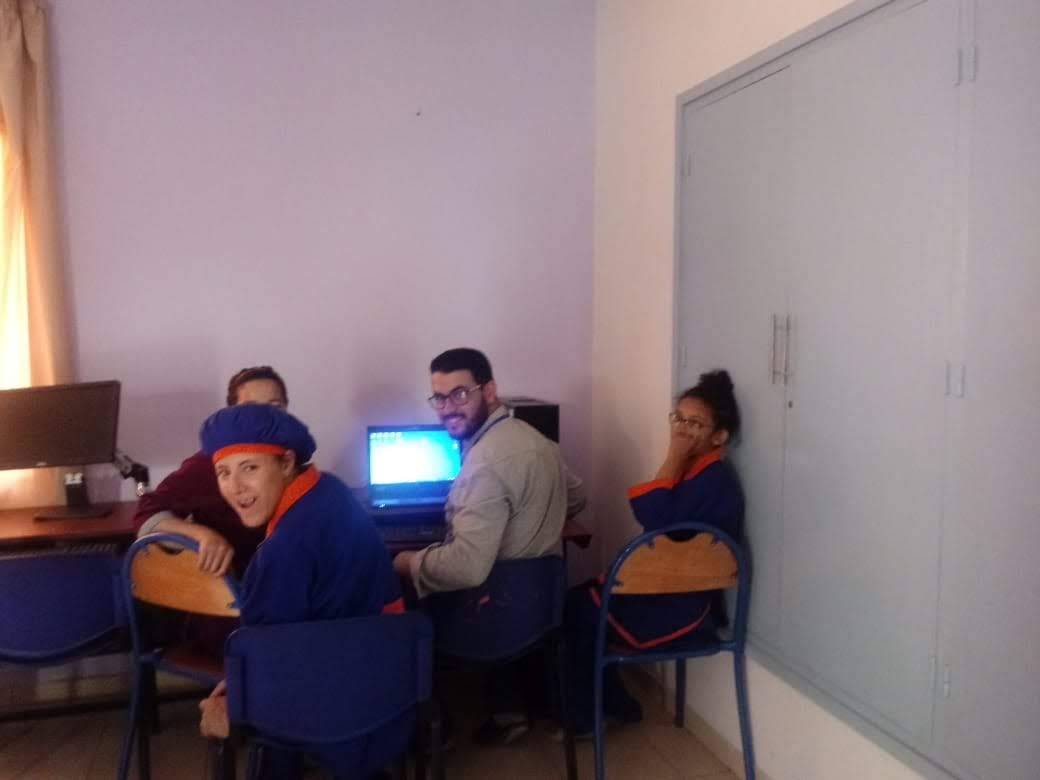
\includegraphics[width=1.2\linewidth,height=170pt]{figures/IMG-20190510-WA0014.jpg}
\end{figure}
			\end{column}
		
		\begin{column}{0.5\linewidth}
 
       \begin{figure}
	\centering
	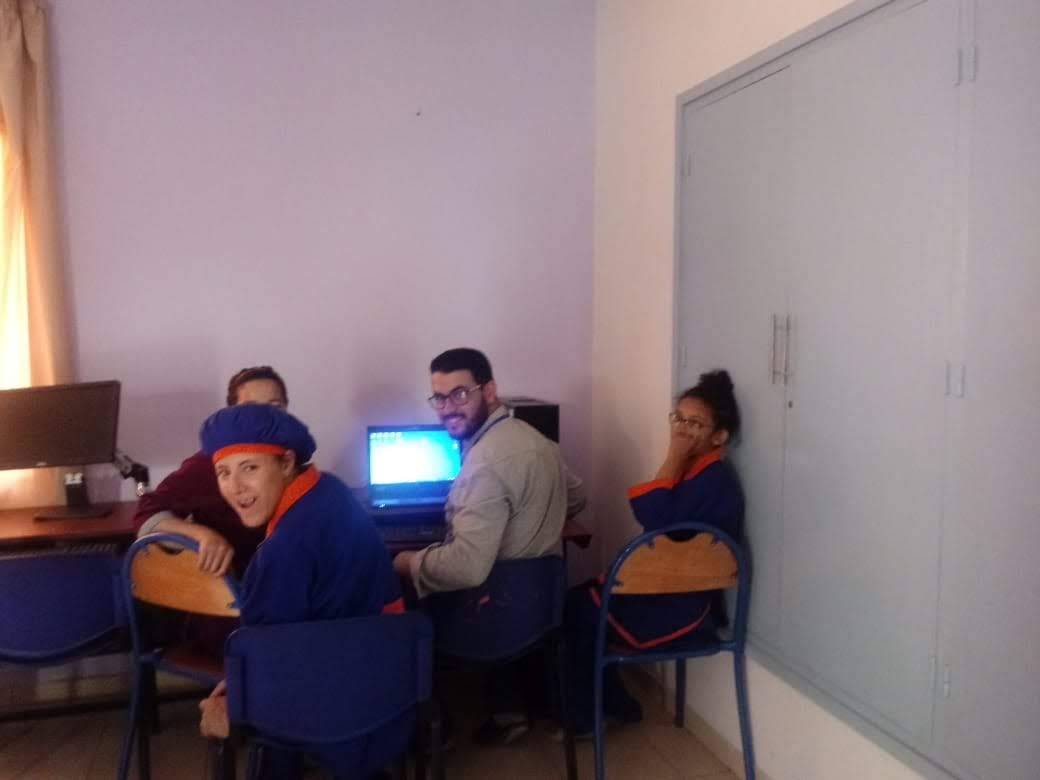
\includegraphics[width=1.2\linewidth,height=170pt]{figures/IMG-20190510-WA0014.jpg}
\end{figure}
			\end{column}
	\end{columns}
	
|
\end{frame}





\begin{frame}{\underline{\secname}}
	
	\begin{center}
		\textbf{Academic background}
	\end{center}
	\begin{columns}
		\begin{column}{0.5\linewidth}
	
	\begin{itemize} 			  \setlength\itemsep{0em}

		\item 2014: High School in Experimental sciences
		\item 2018: B.Sc. in Fundamental Physics
		
		\item 2020: M.Sc. in High energy physics and computational physics first in class 
	\end{itemize}	

			\end{column}
		
	\pause	
		\begin{column}{0.5\linewidth}
		
	\begin{itemize}			  \setlength\itemsep{0em}

		\item 2014: Programming
	\end{itemize}
			\end{column}
	\end{columns}
	\pause
	\begin{center}
	\textbf{Skills}
\end{center}	
	\begin{itemize}			  \setlength\itemsep{0em}
\item
theoretical knowledge in particle physics
\item
Statistics \& probability in HEP 
\item
Programming (C++ \& Python \& ... any OOP language)
% \item
% Object-oriented design (OOD)
% - Abstraction
% Encapsulation
% Inheritance
% Polymorphism
% \item 
% DevOps : Kubernetes + docker + git + Testing and Debugging + Make
% \item 
Soft Skills: Critical Thinking, Effective Communication, Problem solving and logical thinking


% \item
% working with large team project - 
% - Software testing and debugging
% - 
% - Teamwork
% - Communication
% Problem-solving
% Multitasking
% Attention to detail



////////////
As a software engineer at MogulWare, I collaborated with fellow developers on several finance tracker applications for our clients. I used my knowledge of Java and Python to customize functions, troubleshoot issues and debug platforms. I typically managed diverse tasks on seven to eight projects per sprint using a calendar and time tracker to ensure I remained on-schedule with my responsibilities.
//////////////////



“Each day, I spend the first 15 to 30 minutes checking which tasks are left in my sprint, communicating with my supervisor and fellow software engineers to see what tasks are ready for me to start. Then, I prioritize each task based on when it needs to be completed. Finally, I determine how long each task will take and ensure that each task can fit within my hours worked that day.”

Did your research projects involve programming?





Be ready to discuss THEIR work/project

Have an idea of your future plans (where do you see yourself in 5 years..)

Make sure you know and have thought about the STRUCTURE of the programme

		\end{itemize}

\end{frame}




\section{Research Interests \& Experience}


\begin{frame}{\underline{\secname}}

	My correct research interest is in the area of machine learning \& experimental particle physics

	
		\begin{columns}
		\begin{column}{0.5\linewidth}
	
	\begin{itemize} 			  \setlength\itemsep{0em}

		\item symmetry and the standard model (M1 project)
		\item The Standard Model: clifford algebra
		
		
	\end{itemize}	

			\end{column}
		
		\begin{column}{0.5\linewidth}
		
	\begin{itemize}			  \setlength\itemsep{0em}

		\item image equation to latex (NLP)
		\item Breast Cancer Classification (image Classification )
		\item Higgs ML (RNN and xgboost)

	\end{itemize}
			\end{column}
	\end{columns}
	
\vspace{20pt}
	I am available immediately to start an internship before the beginning of the PhD.

	\vspace{20pt}

unfortunately, my master thesis is not related to this PhD position so I worked on a project to show that I am capable to pursue this PhD 





	
\end{frame}


\begin{frame}{\underline{\secname} : My Master Project}
	
	
	\begin{center}
		\textbf{GANs to simulate Drell-Yan  events in  ATLAS experiment}
	\end{center}

	My first use of machine learning but i overcome this problem
	
	
		\begin{itemize}			  \setlength\itemsep{0em}
\item
    Considering a sample of $Z \to \mu \mu$ events in proton-proton collisions, 
    \item
    generated using the {\tt PYTHIA8} event generator at a center-of-mass energy of 13~TeV.
    \item
    Detector resolution and efficiency are taken into account using the parametric description of the ATLAS detector provided by the {\tt DELPHES} detector simulation library.
    \item
    Events are generated with an average of 20 simultaneous collisions (pileup)
	\item
	A rotation of the two four-momenta is applied, so that $p_y^{\mu 1}=0$, after the rotation. Once this is done, $p_y^{\mu 1}$ is discarded from the dataset.
			\end{itemize}

	
	\end{frame}

	
	
\begin{frame}{\underline{\secname} : My Master Project}
	
	
	\begin{center}
		\textbf{GANs to simulate Drell-Yan events in  ATLAS experiment}
	\end{center}


\begin{figure}[H]
	\begin{center}
		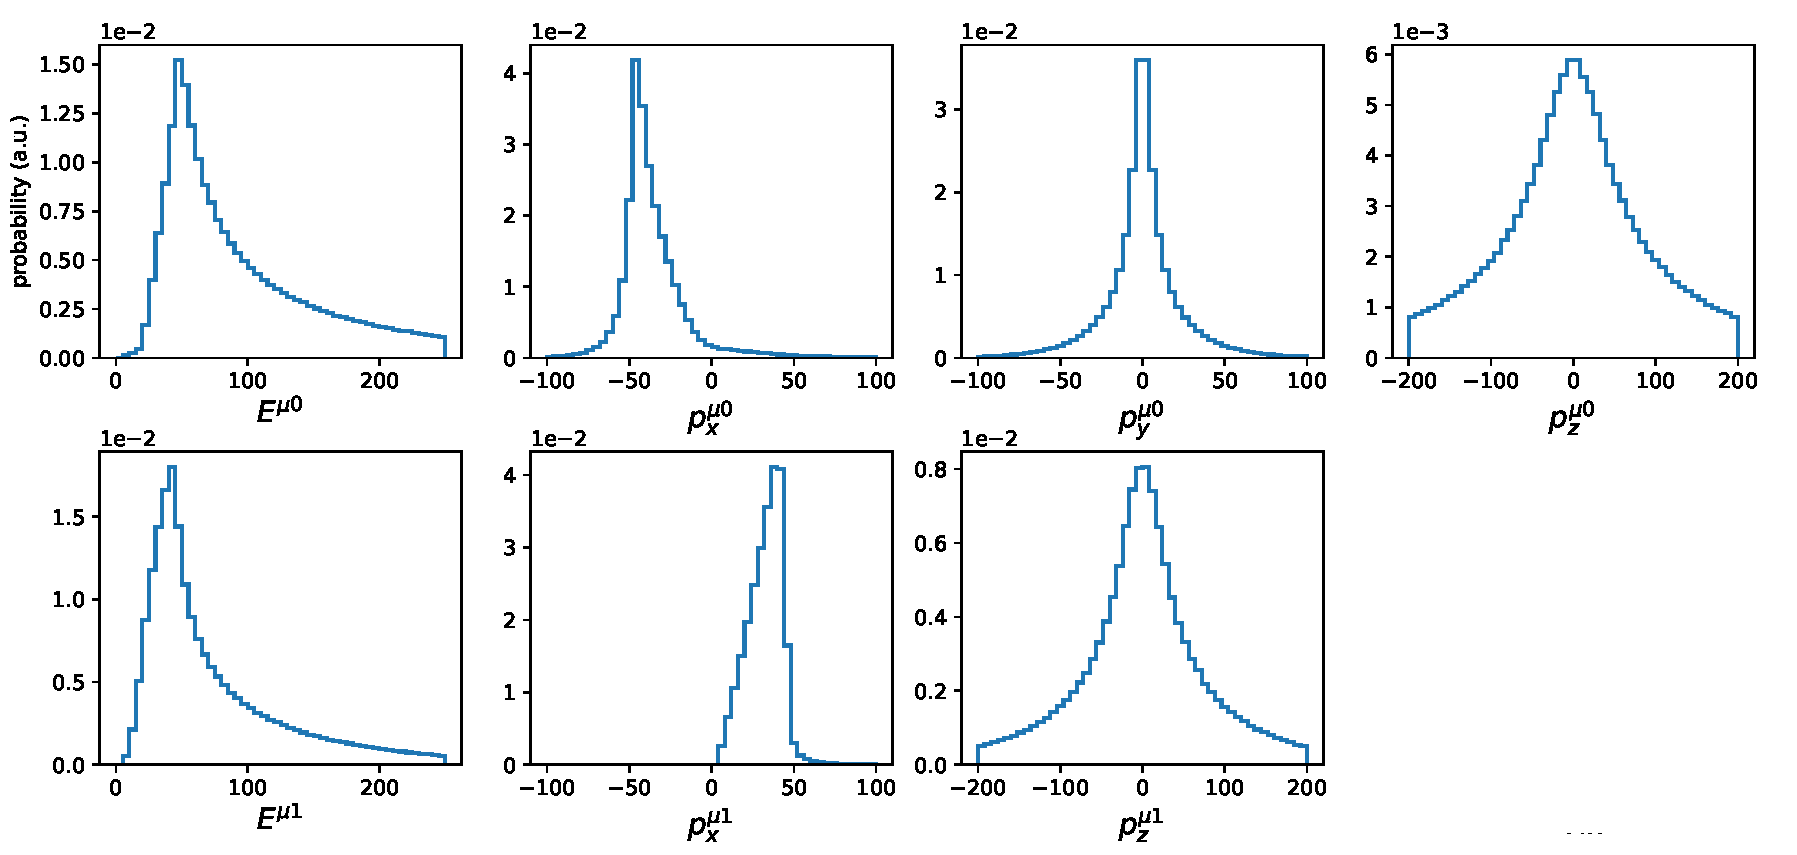
\includegraphics[width=\textwidth]{slides/pdfresizer.com-pdf-crop}
	\end{center}
\end{figure}
	
 \end{frame}



\begin{frame}{\underline{\secname} : My Master Project}
	
	\begin{center}
		\textbf{GANs to simulate Drell-Yan events in  ATLAS experiment}
	\end{center}
			\begin{itemize}			  \setlength\itemsep{0em}
\item
	
	The generator network consists of 7 fully connected layers with 64, 128, 256, 512, 256, 128, 7 neurons. Neurons in the inner layers are activated by leaky ReLU functions, while linear activation functions are used for the output layers. The input to the generator network consists of 7 ``noise'' floating-point numbers, sampled from a Gaussian distribution centered at 0 with unit variance. 
	
	\item

	The discriminator network consists of 9 hidden dense layers with 128, 128, 256, 256, 128, 64, 32, 16, and 8 neurons, activated by a leaky ReLU function. The last hidden layer is fully connected to a single-neuron output layer with sigmoid activation. In addition, a layer connected directly to the input layer returns the dilepton mass as part of the output.
	
\item

The combined network is trained adversarially for 40,000 epochs.

\item

All networks were implemented in {\tt KERAS}, using {\tt TensorFlow} as a back-end, The training was performed using Google TPU type (v2).	
	
				\end{itemize}

 \end{frame}

 
 
\begin{frame}{\underline{\secname} : My Master Project}
	
	
	\begin{center}
		\textbf{GANs to simulate Drell-Yan events in  ATLAS experiment}
	\end{center}	
	
	
\begin{figure}[H]
	\begin{center}
		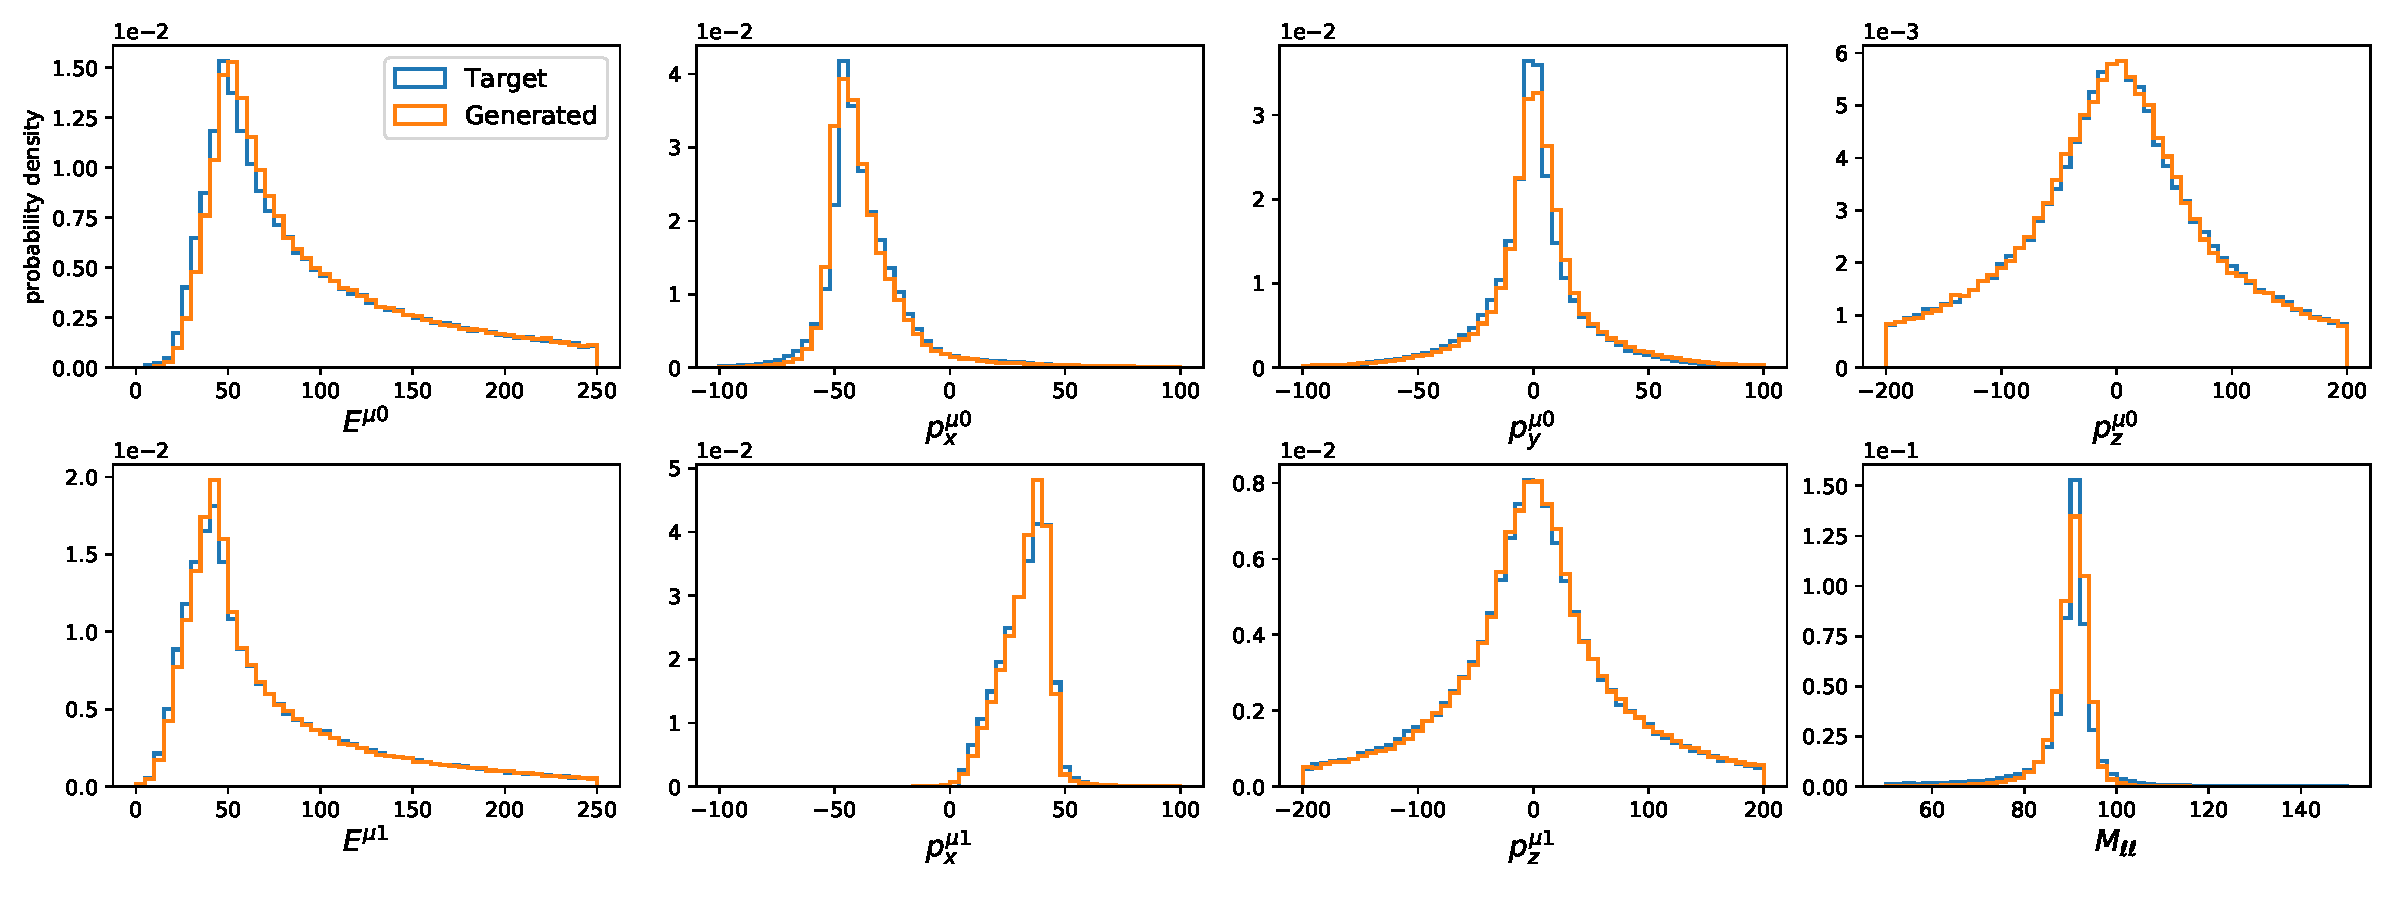
\includegraphics[width=\textwidth]{slides/trial9_epoch39700_minigantest_mllloss_final}
	\end{center}
\end{figure}
	
	


	
\end{frame}

\begin{frame}{\underline{\secname} : My Master Project}
	
	
	\begin{center}
		\textbf{Results}
	\end{center}	
	
			\begin{itemize}			  \setlength\itemsep{0em}
\item
	Results show that GANs can learn the multi-dimensional pdf of $\cal{O}$(7) features
\item
The GAN shows problems in learning distributions with sharp features such as edges
\item
 The Gan indicate a good performance but the reached precision is still insufficient to meet the precision requirements of an LHC data analysis.
			\end{itemize}

 	\begin{center}
		\textbf{Solutions}
	\end{center}
			\begin{itemize}			  \setlength\itemsep{0em}
\item Auxiliary GAN
\item reinforcement learning

\item  Conditional Hybrid GAN


\end{itemize}
\end{frame}




\section{Why this thesis}


\begin{frame}{\underline{\secname}}
	

	\begin{center}
		\textbf{Why this thesis}
	\end{center}
	
	why doing a phd
	why this field
	what set you apart from other candidates
	experience related to this thesis
	why this University  : i love rural cities
	future projects
	your qustions
	
	
	Scientific background and achievements/goals of Honours/Masters project that is being or has been completed. Explanation of techniques used and skills gained
	
	Understanding of the project applied for in terms of scientific background, the challenges it may pose
	
	Why does the student want to do a PhD?
Why this specific PhD - appreciation of the research project objectives
Careers plans for 5-10 years time?
View of the DTP cohort identity of students, cross-partnership events and PIPS placement*
*CASE students are required to spend time with the CASE partner. This obviates the need to arrange a separate PIPS placement 
	
\begin{itemize}
\setlength\itemsep{0em}
\item basics about detector
\item i love computer science physics
\item i worked in many open source projects  with large team
\item i have a good  experience   in working with large team
\item i love germany , i  like working with people from differnet background and culture , devirsity
\end{itemize}

	\begin{center}
		\textbf{}
	\end{center}
	after complete the PhD I plan to pursue a postdoc likely in the area of unsupervised machine learning in data analysis of the ATLAS experiment.
	
\end{frame}








\begin{frame}{\underline{\secname}}
	

	\begin{center}
		\textbf{Why this thesis}
	\end{center}
				\begin{itemize}			  \setlength\itemsep{0em}
\item
I’ve enjoyed my academic work so far, but I really feel I’ve got more to offer as an independent researcher. I’m also passionate about this subject and don’t feel enough attention has been paid to the questions I’m looking to address (appling deep learning to data analysis in lhc big data) .
\item

	
	This thesis combine two of my favorite field: experimental particle physics \& computational physics,
\item
	
I think CEA can help me with these ambitions since it has a strong ATLAS group with access to formidable computational resources.	
\end{itemize}

	\begin{center}
		\textbf{}
	\end{center}
	after complete the PhD I plan to pursue a postdoc likely in the area of unsupervised machine learning in data analysis of the ATLAS experiment.
\end{frame}



%========================
% thanks
%========================


{
%	\usebackgroundtemplate{ \centering \includegraphics[height=\paperheight,width=\paperwidth]{figures/ALICE-pic.pdf}}%
\begin{frame}\frametitle{{\color{white}Finally...}}


\centering

{\vspace{17em} \Huge {\color{white}	\textbf{Thanks For Your Attention !!}\\}}
\end{frame}

}


%=================================================
% end presentation
%=================================================
\end{document}
